\chapter{Analysis}
\label{ch:analysis}
In this chapter we will analyse the data which could occur in an industrial use case,
that includes its structure and amount.
Further we will examine possible workloads for our graph databases in section~\ref{ch:analysis:se:workloads}.

At the end of this chapter in section~\ref{ch:analysis:se:benchmark} we will choose one benchmark for our research.

\section{Data}
\label{ch:analysis:se:data}
As described in section~\ref{ch:background:se:industrialData} we have to work with the data coming from production machines.
Figure~\ref{fig:exampleData} shows us how that data could look like.

Additionally,
our partners at SICK AG~\cite{SICK} gave us the following key data for a product example.
A component carrier with up to 64 circuit boards on it each with up to 128 components is produced every three minutes.
Each component has up to 128 test features.

\subsection{Data Structure}
Looking at the graph in figure~\ref{fig:exampleData} and the example given by SICK we can see that the data looks much like a tree with some cross edges,
a root node at the top and multiple children connected to it with multiple children each.
The given excerpt from figure~\ref{fig:exampleData} shows a part of a testing procedure for a board with components.
Three properties of each component were observed.

We keep this structure in mind for our design in section~\ref{ch:design:se:dataStructure},
where we will compose the structure for our implementation and finally our evaluation.

\subsection{Data Amount}
\label{ch:analysis:se:dataAmount}
To evaluate the amount of data created during production we need to know how much is produced per time unit.
With the parameters mentioned in~\ref{ch:analysis:se:data} we can calculate the maximum number of data points produced every three minutes.

\begin{equation}
  \label{eq:dataAmount}
  \begin{aligned}
    n_{nodes} &= n_{componentCarrier} \\
    &\quad + n_{componentCarrier} \times n_{circuitBoard} \\
    &\quad + n_{componentCarrier} \times n_{circuitBoard} \times n_{component} \\
    &\quad + n_{componentCarrier} \times n_{circuitBoard} \times n_{component} \times n_{test} \\
    \iff &= 1 + 1 \times 64 + 1 \times 64 \times 128 + 1 \times 64 \times 128 \times 128 \\
    \iff &= 1 \times (1 + 64 + 64 \times 128 + 64 \times 128 \times 128) \\
    \iff &= 1 + 64 + 64 \times 128 + 64 \times 128 \times 128 \\
    \iff &= 1 + 64 \times (1 + 128 + 128 \times 128) \\
    \iff &= 1 + 64 \times (1 + 128 \times (1 + 128)) \\
    \iff &= 1 + 64 \times (1 + 128 \times 129) \\
    \iff &= 1 + 64 \times 16.513 \\
    \iff &= 1.056.833
  \end{aligned}
\end{equation}

To calculate the throughput the databases have to archive we need to know how many edges are between the different nodes.
Therefore we need a finished data structure.
In the next chapter in section~\ref{ch:design:se:suitability} we will calculate the target throughput in $ \frac{inserts}{s} $ for the workload design.

In section~\ref{ch:design:se:productionSimulation} we will use these numbers for our workload design.

We can extract the size of each data point from our given example,
each measurement is only two to three characters long,
however the other values range from $ 1 $ to around $ 75 $ characters.
The size for our workload should therefore be in that range.

\section{Workloads}
\label{ch:analysis:se:workloads}
Workloads should represent the mix of operations executed on a database.
There are two main uses for our database in an industrial environment,
the first one is described in section~\ref{ch:analysis:se:insertingData}.
Another one is illustrated in section~\ref{ch:analysis:se:retrievingData}.
The given examples are based on what we think would represent the industrial use of databases.

In section~\ref{ch:design:se:workloads} we will specify our workloads for our evaluation,
the following subsections should only motivate the use for these specific use cases.

\subsection{Inserting Data into the Database}
\label{ch:analysis:se:insertingData}
It is not rare that production runs 24h a day,
therefore data is produced all around the clock.
This shows,
that the ability to store data quickly is a decisive point in choosing a database.
As the machines operate data is continuously written to the database.

\subsection{Retrieving Data from the Database}
\label{ch:analysis:se:retrievingData}
Besides the previous mentioned continuous writing of data into the database,
retrieving data from the database would be the next natural use for it.
That could be in the form of looking up a certain product produced in the past to get its test parameter values or to get all products made by a specific machine to check if some are faulty.

\section{Benchmark Comparison}
\label{ch:analysis:se:benchmark}
To choose a benchmark for our upcoming research we will look at the following aspects of each benchmark.

\begin{itemize}
  \item Data Structure - Of what structure is the generated data?
  \item Workloads - How are the workloads designed?
  \item Programming Language - Is it written in a well-known programming language or do we have to learn it first.
  \item Community - Is there a community for support?
\end{itemize}

The results of our comparison are shown in the following table~\ref{tab:benchmarkComparison}.

\begin{table}[!h]
  \begin{minipage}{\textwidth}
    \begin{tabularx}{\textwidth}{ | l | X | X | X | l | }
      \hline
      Benchmark & Data Structure & Workloads & Programming Language & Community \\ \hline
      Graphalytics & Social Network & Algorithm based & Java & small\footnote{8 contributors and 16 forks on GitHub \url{https://github.com/ldbc/ldbc_graphalytics}} \\ \hline
      YCSB & No specific structure & CRUD based & Java & big\footnote{108 contributors and 1278 forks on GitHub \url{https://github.com/brianfrankcooper/YCSB}} \\ \hline
      XGDBench & Social Network & Read, Update and Graph Traversal & X10 & none\footnote{1 contributor and 1 fork (which is from us) on GitHub \url{https://github.com/miyurud/XGDBench}} \\ \hline
    \end{tabularx}
  \end{minipage}
  \caption{Aspects of the different databases.}
  \label{tab:benchmarkComparison}
\end{table}

Since we are not using a social network structure for our data the graph generators in Graphalytics and XGDBench do not aid us much,
as the generators would be difficult to extend because of their use of complex algorithms to create that structure in the created data~(\cite{Erling2015},~\cite{Dayarathna2012}).
YCSB on the other hand does not serve any particular structure presumably as they are not designed for graph databases and therefore don't need a particular structure on their data.
So YCSB should be easy to extend with our data model.

For the workload aspect Graphalytics uses common algorithms which does not represent out workload scenario.
XGDBench fits our needs better but not quite well, as inserting data is very important for us.
YCSB supports inserting, reading and scanning\footnote{See com.yahoo.ycsb.DB} so it fulfils all our requirements for a benchmark.

Only XGDBench uses another programming language then the other benchmarks namely X10,
which could take some time to learn.

Lastly the community aspect in which YCSB stands out with many contributors and an overall more active community than the other two.

All observed aspects indicate that YCSB would suit our goal the best.
The generator and the workloads should be easily extendable since they have an open design\footnote{See com.yahoo.ycsb.Workload and com.yahoo.ycsb.generator.Generator in \url{https://github.com/brianfrankcooper/YCSB}}.

\section{YCSB}
\label{ch:analysis:se:ycsb}
In this section we will describe the internal workflow of a benchmark run in YCSB.

YCSB separated the execution into two parts.
The first part is the load phase in which the initial data is written to the database.
Then comes the transaction phase where database operations are performed.

Figure~\ref{fig:basicYCSBWorkflow} shows the classes involved in executing a benchmark run with YCSB.
The \texttt{Client} takes the workload file and command-line parameters to set up the database and create \texttt{ClientThreads}.
These \texttt{ClientThreads} call the \texttt{Workload} class to perform an operation on the database,
which is wrapped in the \texttt{DBWrapper}.
Measurements are made through the \texttt{DBWrapper} by stopping the time for every operation made on the database,
it uses the measurements available in the \texttt{measurements} package.

\begin{figure}
  \centering
  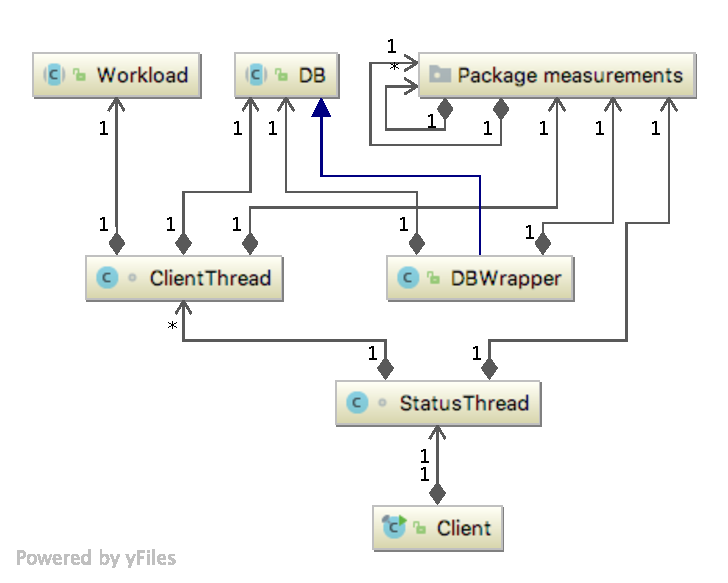
\includegraphics[width=.75\textwidth]{images/benchmarks/basicYCSBWorkflow}
  \caption{Class diagram about the main classes involved in a benchmark run.}
  \label{fig:basicYCSBWorkflow}
\end{figure}

The workload file specifies some parameters about the workload.
These are among others the workload class to use,
how much data should be added in the load phase,
how much operations should be executed in the transaction phase and what percentage of the operations should be inserts, reads, updates, scans or deletes respectively.

The measurements can be saved as histograms each covering one particular operation.
There is also a summary printed out to the console or a file depending on the parameters you set that additionally lists the overall time for the benchmark, operations per second and some more meta information.
